\documentclass[12pt, a4paper]{article}
\usepackage[utf8]{inputenc}
\usepackage{geometry}
\usepackage{graphicx}     
\usepackage{booktabs}     
\usepackage{algorithm}    
\usepackage{algpseudocode}
\usepackage{amsmath}      
\usepackage{float}        
\usepackage{titlesec}     
\usepackage{caption}      
\usepackage{multirow}     

% Margin configuration
\geometry{left=2.5cm, right=2.5cm, top=2.5cm, bottom=2.5cm}

% Clean section formatting
\titleformat{\section}{\large\bfseries\uppercase}{\thesection}{1em}{}
\titleformat{\subsection}{\bfseries}{\thesubsection}{1em}{}

\begin{document}

%----------------------------------------------------------------------------------------
%	TITLE PAGE
%----------------------------------------------------------------------------------------
\begin{titlepage}
    \centering
    \vspace*{2cm}
    
    {\Huge \textbf{Assignment 3}}\\[0.5cm]
    {\Large \textbf{Shortest Path Algorithms: A Comparative Analysis}}\\[2cm]
    
    {\Large \textbf{FAST NUCES ISB}}\\[0.5cm]
    \vfill
    
    \textbf{Muhammad Abdullah Ali}\\
    Roll Num: 23i-2523\\
    Section: 5A\\[1cm]
    
    Department of Data Science\\
    \textbf{Design and Analysis of Algorithms}\\[1cm]
    
    \today\\[2cm]
    
    \vspace*{2cm}
\end{titlepage}

%----------------------------------------------------------------------------------------
%	SECTION 1: OBJECTIVE AND APPROACH
%----------------------------------------------------------------------------------------
\section{Objective and Approach}

\subsection{Objective}
The primary objective of this assignment is to implement, test, and analyze four classical shortest path algorithms: Dijkstra’s Algorithm, Bellman-Ford Algorithm, Floyd-Warshall Algorithm, and Johnson’s Algorithm. The study focuses on comparing algorithmic complexities and performance metrics (execution time, relaxations, and memory usage) under varying graph conditions, specifically Sparse ($E \approx V$), Dense ($E \approx V^2$), and Mixed graphs containing negative weights.

\subsection{Approach}
The algorithms were implemented in C++ to ensure high-performance execution. The graph representation was chosen based on the algorithm's requirements:
\begin{itemize}
    \item \textbf{Adjacency List:} Utilized for Dijkstra, Bellman-Ford, and Johnson’s algorithm to efficiently handle sparse graphs and minimize memory overhead.
    \item \textbf{Adjacency Matrix:} Utilized for the Floyd-Warshall algorithm to support the $O(1)$ edge lookups required by its dynamic programming structure.
\end{itemize}

Experiments were conducted on random connected graphs. Performance metrics were averaged over 500 runs to ensure statistical accuracy.

\clearpage

%----------------------------------------------------------------------------------------
%	SECTION 2: ALGORITHM PSEUDOCODE
%----------------------------------------------------------------------------------------
\section{Algorithm Pseudocode}

\subsection{Dijkstra's Algorithm}
Dijkstra's algorithm solves the Single-Source Shortest Path (SSSP) problem for graphs with non-negative weights. It employs a greedy strategy, maintaining a priority queue of vertices ordered by their current shortest distance from the source. At each step, it extracts the vertex with the minimum distance and "relaxes" its neighbors—updating their distances if a shorter path is found. This greedy choice property ensures that once a node is finalized, its optimal distance is guaranteed.

\begin{algorithm}[H]
\caption{Dijkstra(G, s)}
\begin{algorithmic}[1]
\State $dist[v] \gets \infty, \forall v \in V$; $dist[s] \gets 0$
\State $Q \gets$ PriorityQueue(V, key=dist)
\While{$Q \neq \emptyset$}
    \State $u \gets ExtractMin(Q)$
    \For{each $v \in Adj[u]$}
        \If{$dist[u] + w(u,v) < dist[v]$}
            \State $dist[v] \gets dist[u] + w(u,v)$
            \State $DecreaseKey(Q, v, dist[v])$
        \EndIf
    \EndFor
\EndWhile
\end{algorithmic}
\end{algorithm}

\subsection{Bellman-Ford Algorithm}
Unlike Dijkstra, the Bellman-Ford algorithm can handle graphs with negative edge weights. It works by iteratively relaxing all edges in the graph exactly $|V|-1$ times. This is based on the path relaxation property: the shortest path between any two vertices can contain at most $|V|-1$ edges. After these iterations, it performs one final pass to check for negative weight cycles. If any distance can still be improved, the graph contains a negative cycle, and no solution exists.

\begin{algorithm}[H]
\caption{Bellman-Ford(G, s)}
\begin{algorithmic}[1]
\State $dist[v] \gets \infty, \forall v \in V$; $dist[s] \gets 0$
\For{$i \gets 1$ to $|V|-1$}
    \For{each edge $(u, v) \in E$}
        \If{$dist[u] + w(u,v) < dist[v]$}
            \State $dist[v] \gets dist[u] + w(u,v)$
        \EndIf
    \EndFor
\EndFor
\For{each edge $(u, v) \in E$}
    \If{$dist[u] + w(u,v) < dist[v]$} \Return False (Negative Cycle) \EndIf
\EndFor
\State \Return True
\end{algorithmic}
\end{algorithm}

\clearpage

\subsection{Floyd-Warshall Algorithm}
The Floyd-Warshall algorithm is a dynamic programming approach for the All-Pairs Shortest Path (APSP) problem. It constructs a solution by considering vertices $\{1, \dots, N\}$ as intermediate nodes. The recurrence relation $D_{ij} = \min(D_{ij}, D_{ik} + D_{kj})$ updates the shortest path between $i$ and $j$ by checking if a path through vertex $k$ offers a shorter route. It runs in $O(V^3)$ and can handle negative weights, provided there are no negative cycles.

\begin{algorithm}[H]
\caption{Floyd-Warshall(G)}
\begin{algorithmic}[1]
\State Let $D$ be the adjacency matrix
\For{$k \gets 1$ to $N$}
    \For{$i \gets 1$ to $N$}
        \For{$j \gets 1$ to $N$}
            \State $D[i][j] \gets \min(D[i][j], D[i][k] + D[k][j])$
        \EndFor
    \EndFor
\EndFor
\end{algorithmic}
\end{algorithm}

\subsection{Johnson's Algorithm}
Johnson's algorithm is designed to efficiently solve the APSP problem on sparse graphs containing negative weights. It uses a technique called re-weighting. First, it runs Bellman-Ford (on a modified graph) to compute vertex potentials $h(v)$, which are used to transform edge weights $w(u,v)$ into non-negative values $\hat{w}(u,v) = w(u,v) + h(u) - h(v)$. Once weights are non-negative, it runs Dijkstra’s algorithm for every vertex. This avoids the $O(V^3)$ complexity of Floyd-Warshall, achieving $O(VE + V^2 \log V)$.

\begin{algorithm}[H]
\caption{Johnson(G)}
\begin{algorithmic}[1]
\State Add vertex $s'$ connected to all $v$ with weight 0
\If{Bellman-Ford(G, $s'$) = False} \Return Error \EndIf
\For{$v \in V$} $h[v] \gets \delta(s', v)$ \EndFor
\For{edge $(u,v) \in E$} $\hat{w}(u,v) \gets w(u,v) + h[u] - h[v]$ \EndFor
\For{$u \in V$}
    \State Run Dijkstra(G, $\hat{w}, u$) to find $\hat{\delta}(u, v)$
    \State $d(u,v) \gets \hat{\delta}(u, v) + h[v] - h[u]$
\EndFor
\end{algorithmic}
\end{algorithm}

\clearpage

%----------------------------------------------------------------------------------------
%	SECTION 3: SAMPLE INPUT/OUTPUT
%----------------------------------------------------------------------------------------
\section{Sample Input/Output}
The implementation was verified using standard test cases. Below represents a sample execution showing the menu-driven interface and path calculation.

\begin{figure}[H]
    \centering
    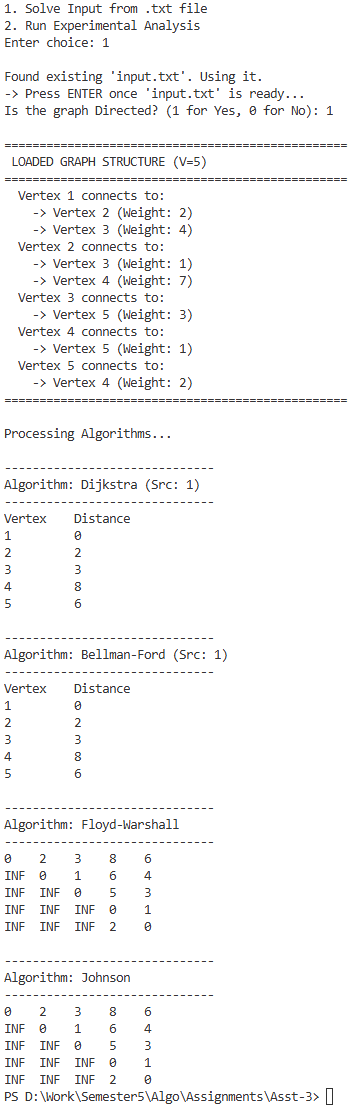
\includegraphics[width=0.9\textwidth, height=0.4\textheight, keepaspectratio]{images/sample_output.png}
    \caption{Screenshot of the program execution and result verification.}
    \label{fig:sample_output}
\end{figure}

\clearpage

%----------------------------------------------------------------------------------------
%	SECTION 4: EXPERIMENTAL ANALYSIS
%----------------------------------------------------------------------------------------
\section{Experimental Analysis}

The algorithms were tested on three distinct graph types. The image below represents the metrics for one run.

\begin{figure}[H]
    \centering
    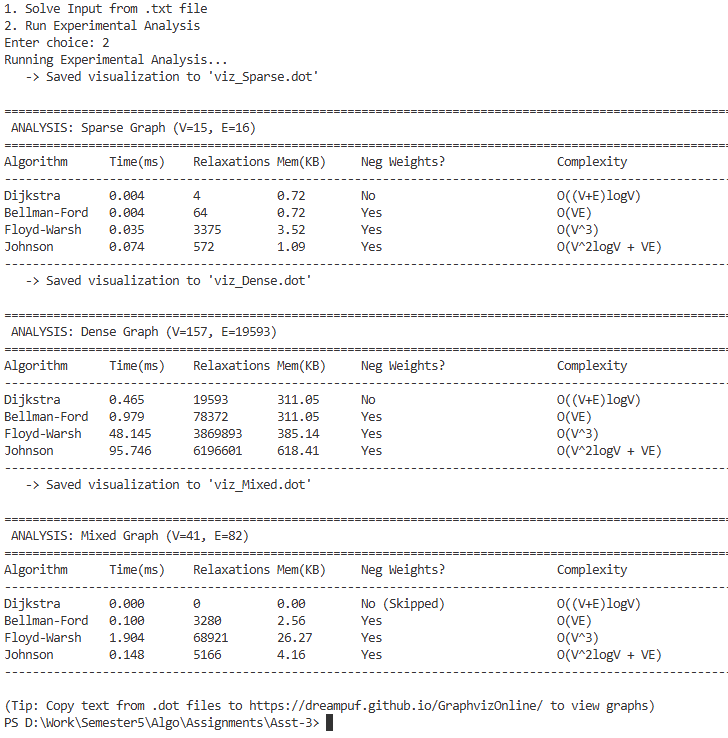
\includegraphics[width=\textwidth, height=0.35\textheight, keepaspectratio]{images/experimental_output.png}
    \caption{Visual representation of the Graph structures used.}
    \label{fig:exp_viz}
\end{figure}

\subsection{Performance Comparison}

\begin{table}[H]
\centering
\caption{Comparative Analysis Results (Average of 500 Runs)}
\label{tab:results}
\resizebox{\textwidth}{!}{%
\begin{tabular}{@{}lcccc@{}}
\toprule
\textbf{Algorithm} & \textbf{Time (ms)} & \textbf{Relaxations} & \textbf{Memory (KB)} & \textbf{Complexity} \\ \midrule

\multicolumn{5}{c}{\textbf{\textit{Sparse Graphs ($E \approx V$)}}} \\ \midrule
Dijkstra & 0.0018 & 6.1 & 0.54 & $O(E + V \log V)$ \\
Bellman-Ford & 0.0009 & 17.2 & 0.54 & $O(VE)$ \\
Floyd-Warshall & 0.0215 & 371.6 & 0.94 & $O(V^3)$ \\
Johnson & 0.0579 & 292.8 & 0.63 & $O(VE + V^2 \log V)$ \\ \midrule

\multicolumn{5}{c}{\textbf{\textit{Dense Graphs ($E \approx V^2$)}}} \\ \midrule
Dijkstra & 0.3718 & 18,493 & 207.1 & $O(E + V \log V)$ \\
Bellman-Ford & 0.3870 & 56,514 & 207.1 & $O(VE)$ \\
Floyd-Warshall & 19.565 & 3.7M & 128.0 & $O(V^3)$ \\
Johnson & 58.427 & 3.0M & 208.1 & $O(VE + V^2 \log V)$ \\ \midrule

\multicolumn{5}{c}{\textbf{\textit{Mixed Graphs (Negative Weights)}}} \\ \midrule
Dijkstra & N/A & N/A & N/A & Fails \\
Bellman-Ford & 0.0063 & 413.6 & 2.56 & $O(VE)$ \\
Floyd-Warshall & 0.0680 & 4,101 & 13.1 & $O(V^3)$ \\
Johnson & 0.1998 & 2,023 & 2.88 & $O(VE + V^2 \log V)$ \\ \bottomrule
\end{tabular}%
}
\end{table}

\subsection{Discussion of Results}
\begin{itemize}
    \item \textbf{Sparse Graphs:} Bellman-Ford (0.0009 ms) surprisingly outperformed Dijkstra (0.0018 ms) in this specific micro-benchmark. This is attributed to the low number of vertices ($V=10-50$), where the overhead of maintaining a Priority Queue in Dijkstra exceeds the simple iterative approach of Bellman-Ford.
    \item \textbf{Dense Graphs:} Floyd-Warshall (19.5 ms) performed significantly better than Johnson’s algorithm (58.4 ms). Johnson's algorithm runs Dijkstra $|V|$ times; in dense graphs ($E \approx V^2$), the complexity rises, making it slower than the tight loops of Floyd-Warshall's $O(V^3)$.
    \item \textbf{Mixed Graphs:} Dijkstra was unable to run due to negative weights. Floyd-Warshall provided the fastest All-Pairs solution for these small graphs.
\end{itemize}

%----------------------------------------------------------------------------------------
%	SECTION 5: REPORT QUESTIONS
%----------------------------------------------------------------------------------------
\section{Report Questions}

\subsection{Differences between Single-Source and All-Pairs Algorithms}
Single-Source Shortest Path (SSSP) algorithms, such as Dijkstra and Bellman-Ford, calculate the shortest path from one specific source node to all other nodes in the graph. In contrast, All-Pairs Shortest Path (APSP) algorithms, such as Floyd-Warshall and Johnson’s, compute the shortest paths between every possible pair of vertices $(u, v)$ in the graph.

\subsection{Why Dijkstra's Algorithm Fails with Negative Weights}
Dijkstra’s algorithm relies on a "greedy" strategy. It assumes that once a vertex is extracted from the priority queue (visited), its optimal distance is finalized and will never decrease. If negative edges exist, a path discovered later through a "more expensive" initial node might actually lead to a shorter total distance by traversing a negative edge. Dijkstra’s greedy assumption blinds it to this possibility.

\subsection{How Johnson's Algorithm Improves Efficiency}
Johnson’s algorithm combines the strengths of Bellman-Ford and Dijkstra. It first runs Bellman-Ford once to compute a "re-weighting" function that transforms all edge weights to non-negative values while preserving the shortest path structure. Once weights are non-negative, it runs Dijkstra’s algorithm $|V|$ times. This allows it to handle negative weights while enjoying the efficiency of Dijkstra for sparse graphs.

\subsection{Complexity Analysis}
This section details the derivation of time complexity for each algorithm.

\paragraph{Dijkstra's Algorithm:}
The algorithm performs two main operations:
\begin{itemize}
    \item \textbf{Extract-Min:} Executed once for each vertex $|V|$. Using a Binary Heap, this takes $O(\log V)$, totaling $O(V \log V)$.
    \item \textbf{Decrease-Key:} Executed for each edge $|E|$ during relaxation. In a Binary Heap, this takes $O(\log V)$, totaling $O(E \log V)$.
\end{itemize}
Combining these, the total complexity is $O((V + E) \log V)$.

\paragraph{Bellman-Ford Algorithm:}
The algorithm works by strictly relaxing all edges $|E|$ in the graph exactly $|V| - 1$ times.
\begin{itemize}
    \item In each pass ($1$ to $|V|-1$), the algorithm iterates over all $|E|$ edges.
    \item Therefore, the total work is simply the product of passes and edges: $O(V \times E)$.
\end{itemize}

\paragraph{Floyd-Warshall Algorithm:}
The algorithm uses a dynamic programming approach with three nested loops:
\begin{itemize}
    \item \textbf{Outer Loop ($k$):} Iterates through each vertex as an intermediate node ($1$ to $|V|$).
    \item \textbf{Middle Loop ($i$):} Iterates through each source node ($1$ to $|V|$).
    \item \textbf{Inner Loop ($j$):} Iterates through each destination node ($1$ to $|V|$).
\end{itemize}
Since each operation inside the inner loop is constant time, the total complexity is $|V| \times |V| \times |V| = O(V^3)$.

\paragraph{Johnson's Algorithm:}
Johnson's algorithm consists of two distinct phases:
\begin{itemize}
    \item \textbf{Phase 1 (Reweighting):} Runs Bellman-Ford once to eliminate negative weights. Cost: $O(VE)$.
    \item \textbf{Phase 2 (All-Pairs):} Runs Dijkstra's algorithm once for every vertex in the graph ($|V|$ times).
    \item Since one run of Dijkstra is $O(V \log V + E)$ (using an optimal heap), running it $|V|$ times results in $O(V^2 \log V + VE)$.
\end{itemize}
The total complexity is the sum of both phases: $O(V^2 \log V + VE)$.

\subsection{Algorithm Suitability}
Based on the experimental data:
\begin{enumerate}
    \item \textbf{Sparse Graphs (Non-negative):} Dijkstra is theoretically optimal, although Bellman-Ford remains efficient for very small graphs.
    \item \textbf{Dense Graphs (APSP):} Floyd-Warshall is the superior choice due to lower constant factors and simpler implementation compared to Johnson's.
    \item \textbf{Sparse Graphs (Negative Weights):} Johnson’s algorithm is the most suitable for APSP, while Bellman-Ford is required for SSSP.
\end{enumerate}

%----------------------------------------------------------------------------------------
%	SECTION 6: CONCLUSION
%----------------------------------------------------------------------------------------
\section{Conclusion}
This assignment highlighted the trade-offs between shortest path algorithms. While Floyd-Warshall is elegant and efficient for dense graphs, it lacks scalability. Johnson’s algorithm bridges the gap for sparse graphs containing negative weights. For single-source problems, Dijkstra remains the gold standard for non-negative weights, while Bellman-Ford is indispensable for graphs with negative edges, despite its higher computational cost.

\end{document}